\documentclass[11pt, letterpaper]{article}
\input{/home/hyperion/.config/LatexHub/preambles/base.tex}
\input{/home/hyperion/.config/LatexHub/preambles/diagrams.tex}
\input{/home/hyperion/.config/LatexHub/preambles/tikz.tex}
\input{/home/hyperion/.config/LatexHub/preambles/macros-cat-theory.tex}
\input{/home/hyperion/.config/LatexHub/preambles/macros-algebra.tex}
\input{/home/hyperion/.config/LatexHub/preambles/basic-theorems-section.tex}
\input{/home/hyperion/.config/LatexHub/preambles/refs-basic.tex}
\input{/home/hyperion/.config/LatexHub/preambles/code.tex}
\theoremstyle{plain}
\newtheorem{problem}{Problem}[section]


\usepackage{titlesec}
\titleformat{\section}{\normalfont\Large\bfseries}{}{0em}{}
\usepackage{titlepageBU}
\title{Homework 2}
\begin{document}
\makeproblem

\section{Problem 1}
\begin{problem}
	Consider a particle with constant acceleration in the $z$ direction, which begins at rest at $z=0$ at $t=0$. Relativistically, the acceleration is the time derivative of momemtum $p=\gamma v$, so the equation of motion is
	\[
		\frac{\mathrm{d}p_z}{\mathrm{d}t} =-a
	\]
	where $a$ is constant and $\gamma =\left( 1-v^2 \right) ^{-1/2} $, $v=\dot{z} $. Solve $\dot{z} $ for $z(t)$, and use this to find $\frac{\mathrm{d}\tau }{\mathrm{d}t} $. Finally, obtain $U^\mu =\left( \frac{\mathrm{d}t}{\mathrm{d}\tau } ,\frac{\mathrm{d}x}{\mathrm{d}\tau } ,\frac{\mathrm{d}y}{\mathrm{d}\tau } ,\frac{\mathrm{d}z}{\mathrm{d}\tau }  \right) =\frac{\mathrm{d}x^\mu }{\mathrm{d}\tau } $ as a function of $t$.
\end{problem}
\noindent\textbf{Solution.}
\[
	\int -a \,\mathrm{d} t=\int \frac{\mathrm{d}p_z}{\mathrm{d}t}  \,\mathrm{d} t\implies p_z(t)=-at +C
.\]
The constant of integration vanishes since $v=0$ at $t=0$ implies $p_z(0)=0$. We then use $p=\gamma v$ to obtain
\[
	-at=\frac{v}{\sqrt{1-v^2} } \implies a^2t^2\left( 1-v^2 \right) =v^2\implies \left( 1+a^2t^2 \right) v^2=a^2t^2
.\]
This gives us
\[
	v=-\sqrt{\frac{a^2t^2}{a^2t^2+1} } =-\frac{at}{\sqrt{a^2t^2+1} } 
.\]
There was a negative sign there before so we bring it back when taking the square root. Integrating gives
\[
	z(t)=\int \frac{\mathrm{d}z}{\mathrm{d}t}  \,\mathrm{d} t=\int -\frac{at}{\sqrt{a^2t^2+1} }  \,\mathrm{d} t
.\]
Substitute $u=a^2t^2+1$. Then this equals
\[
	=-\int \frac{1}{2a} \frac{1}{\sqrt{u} }  \,\mathrm{d} u=-\frac{1}{2a} \int u^{-1/2}  \,\mathrm{d} u=-\frac{1}{2a} 2\sqrt{u} +C=-\frac{\sqrt{a^2t^2+1} }{a} +C
.\]
Imposing initial conditions gives
\[
	-\frac{1}{a} +C=0\implies C=\frac{1}{a} 
.\]
Therefore,
\[
	z(t)=\frac{1}{a} \left( 1-\sqrt{a^2t^2+1} \right) 
.\]

To solve for $\frac{\mathrm{d}\tau }{\mathrm{d}t} $, recall that $\mathrm{d} \tau ^2=-\eta _{\mu \nu } \mathrm{d} x^\mu \mathrm{d} x^\nu $. In flat space (which I assume we are in?) this is
\[
	\mathrm{d} \tau ^2=\mathrm{d} t^2-\mathrm{d} x^2-\mathrm{d} y^2-\mathrm{d} z^2
.\]
We recover
\[
	\frac{\mathrm{d}\tau }{\mathrm{d}t} ^2=\frac{\mathrm{d}t}{\mathrm{d}t} ^2-\frac{\mathrm{d}x}{\mathrm{d}t} ^2-\frac{\mathrm{d}y}{\mathrm{d}t} ^2-\frac{\mathrm{d}z}{\mathrm{d}t}^2 =1-\left( \frac{\mathrm{d}x^i}{\mathrm{d}t} ^2 \right) =1-\left( v_x^2+v_y^2+v_z^2 \right) =1-\left| v \right| ^2
.\]
We then obtain
\[
	\frac{\mathrm{d}\tau }{\mathrm{d}t} =\sqrt{1-\left| v \right| ^2} 
.\]
Since $v$ is zero in this frame except in the $z$-component by assumption, $\left| v \right| ^2=v_z^2$, which we will continue writing as $v^2$ for simplicity. This gives us that $\frac{\mathrm{d}\tau }{\mathrm{d}t} =\sqrt{1-v^2} $. Note that this is precisely $1/\gamma $. Using our formula
\[
	v=-\frac{at}{\sqrt{a^2t^2+1} } ,
\]
we obtain
\[
	\frac{\mathrm{d}\tau }{\mathrm{d}t}=\sqrt{1-\frac{a^2t^2}{a^2t^2+1} } =\sqrt{\frac{a^2t^2+1-a^2t^2}{a^2t^2+1} } =\sqrt{\frac{1}{a^2t^2+1} } =\frac{1}{\sqrt{a^2t^2+1} } 
.\]

To compute $U^\mu $, recall that (or do the 1-line proof via chain rule)
\[
	\frac{\mathrm{d}t}{\mathrm{d}\tau } =\frac{1}{\mathrm{d} \tau /\mathrm{d} t} =\sqrt{a^2t^2+1} 
.\]
We also have
\[
	\frac{\mathrm{d}z}{\mathrm{d}\tau } =\frac{\mathrm{d}z}{\mathrm{d}t} \frac{\mathrm{d}t}{\mathrm{d}\tau } =-\frac{at}{\sqrt{a^2t^2+1} } \sqrt{a^2t^2+1} =-at
.\]
An alternative way to see this is
\[
	\frac{\mathrm{d}z}{\mathrm{d}t} \frac{\mathrm{d}t}{\mathrm{d}\tau } =v\gamma =p_z
.\]
Since $v_x=v_y=0$, we have
\[
	\frac{\mathrm{d}x}{\mathrm{d}\tau } =\frac{\mathrm{d}x}{\mathrm{d}t} \frac{\mathrm{d}t}{\mathrm{d}\tau } =0\sqrt{a^2t^2+1} =0,
\]
and the same with $\frac{\mathrm{d}y}{\mathrm{d}\tau } $. As a quick sanity check,
\[
	1=\frac{\mathrm{d}\tau }{\mathrm{d}\tau } ^2=\frac{\mathrm{d}t}{\mathrm{d}\tau } ^2-\frac{\mathrm{d}x}{\mathrm{d}\tau } ^2-\frac{\mathrm{d}y}{\mathrm{d}\tau } ^2-\frac{\mathrm{d}z}{\mathrm{d}\tau } ^2=\sqrt{a^2t^2+1} ^2-(-at)^2=a^2t^2+1-a^2t^2=1
.\]
Therefore,
\[
	U^\mu =\left( \sqrt{a^2t^2+1} ,0,0,-at \right) 
.\]


\section{Problem 2}

\begin{problem}
	Consider a particle of charge-to-mass ratio $q/m=1$ in an accelerating universe with $a(t)=e^t$, in the background of a constant electric field $E^i$ in the $z$ direction, $E^i=E_0\delta _3^i$. If the particle is at rest at the origin at time 0 $(x^\mu =0)$, then find the trajectory of the particle numerically when $E_0=1/2$ and plot $z$ as a function of $t$.
\end{problem}
In locally inertial coordinates, we defined
\[
	F^{0i} =E^i,\qquad F^{ij} =\varepsilon ^{ijk} B_k
.\]
Since we are in the absense of a magnetic field, the terms $F^{\mu \nu } $ with $\mu \neq 0$ vanish. Using our definition, this takes the matrix form
\[
	F^{\mu \nu } =\begin{pmatrix}
	0 & 0 & 0 & E_0 \\
	0 & 0 & 0 & 0 \\
	0 & 0 & 0 & 0 \\
	-E_0 & 0 & 0 & 0
	\end{pmatrix}
.\]

In the expanding universe, the line element is given by
\[
	\mathrm{d} s^2=-\mathrm{d} t^2+a(t)^2\left( \mathrm{d} x^2+\mathrm{d} y^2+\mathrm{d} z^2 \right) = g_{\mu \nu } \mathrm{d} x^\mu \mathrm{d} x^\nu 
.\]
Using $a(t)=e^t$, we then see that the metric is given by
\[
	g_{\mu \nu } =\operatorname{diag} (-1,e^{2t} ,e^{2t} ,e^{2t})
.\]
The transformation law is given by
\[
	F^{\mu \nu } =\frac{\partial x^\mu }{\partial (x')^\alpha } \frac{\partial x^\nu }{\partial (x')^\beta } F^{\prime \alpha \beta } 
.\]
Here we take $x^\mu $ is our coordinate system in the metric $g_{\mu \nu } $ and $(x')^\mu $ are our locally inertial coordinates. The transformation law is simple to obtain:
\[
	e^{2t}\mathrm{d} x^2=\mathrm{d} x^{\prime 2} \implies e^t \mathrm{d} x=\mathrm{d} x'\implies \frac{\mathrm{d}x}{\mathrm{d}x'} =\frac{1}{e^t} 
.\]
The same shows that
\[
	\frac{\mathrm{d}y}{\mathrm{d}y'} =\frac{1}{e^t},\qquad \frac{\mathrm{d}z}{\mathrm{d}z'} =\frac{1}{e^t} 
.\]
We also have $\mathrm{d} t^2=\mathrm{d} t^{\prime 2} $ implies that
\[
	\frac{\mathrm{d}t}{\mathrm{d}t'} =1
.\]
The Jacobian then takes the form
\[
	J^{\mu }_\nu =\frac{\partial x^\mu }{\partial x^{\prime \nu } } =\begin{pmatrix}
	1 &  &  &  \\
	 & e^{-t}  &  &  \\
	 &  & e^{-t}  &  \\
	 &  &  & e^{-t} 
	\end{pmatrix}
.\]
Then
\[
	F^{\mu \nu } =J^\mu_\alpha F^{\prime \alpha \nu } \left(J^{\nu }_\beta \right)^T-\begin{pmatrix}
	1 &  &  &  \\
	 & e^{-t}  &  &  \\
	 &  & e^{-t}  &  \\
	 &  &  & e^{-t} 
	\end{pmatrix}\begin{pmatrix}
	 &  &  & E_0 \\
	 &  &  &  \\
	 &  &  &  \\
	-E_0 &  &  & 
	\end{pmatrix}\begin{pmatrix}
	1 &  &  &  \\
	 & e^{-t}  &  &  \\
	 & & e^{-t}  &  \\
	 &  &  & e^{-t} 
	\end{pmatrix}
\]
\[
	=\begin{pmatrix}
	 &  &  & E_0 \\
	 &  &  &  \\
	 &  &  &  \\
	-E_0e^{-t}  &  &  & 
	\end{pmatrix}\begin{pmatrix}
	1 &  &  &  \\
	 & e^{-t}  &  &  \\
	 &  & e^{-t}  &  \\
	 &  &  & e^{-t} 
	\end{pmatrix}=\begin{pmatrix}
	 &  &  & E_0e^{-t}  \\
	 &  &  &  \\
	 &  &  &  \\
	-E_0e^{-t}  &  &  & 
	\end{pmatrix}
.\]
We have found $F^{\mu \nu } $ in the expanding universe coordinate system.

Recall from equation 6.2.16 in the notes that a particle in an electric field $\vec{E} $ and magnetic field $\vec{B} $ obeys the equation of motion
\[
	\frac{\mathrm{D} }{\mathrm{d} \tau } \frac{\mathrm{d}x^\mu }{\mathrm{d}\tau } =\frac{q}{m} F^\mu\!_\nu \frac{\mathrm{d}x^\nu }{\mathrm{d}\tau } =F^\mu \!_\nu \frac{\mathrm{d}x^\nu }{\mathrm{d}\tau } 
.\]
We have
\[
	\frac{\mathrm{d}x^\alpha }{\mathrm{d}\tau  } \nabla_\alpha \frac{\mathrm{d}x^\mu }{\mathrm{d}\tau }=F^\mu \!_\nu \frac{\mathrm{d}x^\nu }{\mathrm{d}\tau } 
.\]
Writing $U^\mu =\frac{\mathrm{d}x^\mu }{\mathrm{d}\tau } $ for the 4-velocity in proper time and expanding the covariant derivative yields
\[
	\frac{\mathrm{d}x^\alpha }{\mathrm{d}\tau } \left( \frac{\partial U^\mu }{\partial x^\alpha } +\Gamma ^\mu_{\alpha \sigma } U^\sigma  \right) =F^\mu \!_\nu U^\nu =g_{\nu \alpha } F^{\mu \alpha } U^\nu 
.\]
We now need to compute the Christoffel symbols. I decided I wanted to just directly compute them from
\[
	\Gamma_{\alpha \sigma } ^\mu= \frac{1}{2} g^{\rho \mu } \left( \frac{\partial g_{\alpha \rho } }{\partial x^\sigma } +\frac{\partial g_{\sigma \rho } }{\partial x^\alpha } -\frac{\partial g_{\alpha \sigma } }{\partial x^\rho }  \right) 
.\]
Since $g^{\rho \mu } $ is the inverse of the metric, we have $g^{\rho \nu } =\operatorname{diag} (-1,e^{-2t} ,e^{-2t} ,e^{-2t} )$. Since the off-diagonal terms vanish, we only get contributions when $\rho =\mu $, so
\[
	\Gamma^\mu_{\alpha \sigma } =\frac{1}{2} g^{\mu \mu } \left( \frac{\partial g_{\alpha \mu } }{\partial x^\sigma } +\frac{\partial g_{\sigma \mu } }{\partial x^\alpha } -\frac{\partial g_{\alpha \sigma } }{\partial x^\mu }  \right) 
.\]
Since the components of $g_{\mu \nu } $ only have time-dependence, any derivative with respect to a spatial coordinate vanishes. In other words, $\frac{\partial g_{\mu \nu } }{\partial x^\sigma } =\frac{\partial g_{\mu \nu } }{\partial t} $. This simplifies everything considerably.

\[
	\Gamma ^0_{\alpha \sigma } =-\frac{1}{2} \left( \frac{\partial g_{\alpha 0} }{\partial x^\sigma } +\frac{\partial g_{\sigma 0} }{\partial x^\alpha } -\frac{\partial g_{\alpha \sigma } }{\partial t}  \right) 
.\]
We get a contribution from the first partial when $\alpha=0$ and $\sigma =0$, we get a contribution from the second when $\sigma =0$ and $\alpha =0$, and we get a contribution from the final one when $\alpha =\sigma $. We start with
\[
	\Gamma^0_{00} =-\frac{1}{2} \left( \frac{\partial (-1)}{\partial t} +\frac{\partial (-t)}{\partial t}-\frac{\partial (-1)}{\partial t}  \right) =0
.\]
The first two partials vanish for the other cases, so we have
\[
	\Gamma ^0_{\alpha \alpha } =\frac{1}{2} \frac{\partial g_{\alpha \alpha } }{\partial t}
.\]
Since $g_{\alpha \alpha } =e^{2t} $ for $\alpha \neq 0$, we have
\[
	\Gamma^0_{\alpha \sigma } =\begin{pmatrix}
	 0& 0 & 0 & 0 \\
	0 & e^{2t}  & 0 & 0 \\
	0 & 0 & e^{2t}  & 0 \\
	0 & 0 & 0 & e^{2t} 
	\end{pmatrix}
.\]
We still only get contributions from time derivatives, so the final derivative vanishes for all other cases since $\mu \neq 0$.
\[
	\Gamma ^1_{\alpha \sigma } =\frac{e^{-2t} }{2} \left( \frac{\partial g_{\alpha 1} }{\partial x^\sigma } +\frac{\partial g_{\sigma 1} }{\partial x^\alpha }  \right) 
.\]
This only gets contributions when $(\alpha ,\sigma )=(1,0)$ or $(0,1)$. We compute
\[
	\Gamma ^1_{10} =\frac{e^{-2t} }{2} \left( \frac{\partial g_{11} }{\partial t} +\frac{\partial g_{01} }{\partial x}  \right) =\frac{e^{-2t} }{2} \frac{\partial }{\partial t} e^{2t} =1
,\]
\[
	\Gamma ^1_{01} =\Gamma ^1_{10} =1
.\]
\[
	\Gamma ^1_{\alpha \sigma } =\begin{pmatrix}
	0 & 1  & 0 & 0 \\
	1  & 0 & 0 & 0 \\
	0 & 0 & 0 & 0 \\
	0 & 0 & 0 & 0
	\end{pmatrix}
.\]
We similarly see that
\[
	\Gamma ^2_{\alpha \sigma } =\frac{e^{-2t} }{2} \left( \frac{\partial g_{\alpha 2} }{\partial x^\sigma } +\frac{\partial g_{\sigma 2} }{\partial \alpha }  \right) 
\]
vanishes unless $2=\alpha $ and $\sigma =0$, or the converse case. This gives
\[
	\Gamma ^2_{20} =\frac{e^{-2t} }{2} \frac{\partial e^{2t} }{\partial t} =1=\Gamma ^2_{02} 
,\]
and thus
\[
	\Gamma ^2_{\alpha \sigma } =\begin{pmatrix}
	0 & 0 & 1 & 0 \\
	0 & 0 & 0 & 0 \\
	1 & 0 & 0 & 0 \\
	0 & 0 & 0 & 0
	\end{pmatrix}
.\]
It is at this point clear that
\[
	\Gamma^3_{\alpha \sigma } =\begin{pmatrix}
	0 & 0 & 0 & 1 \\
	0 & 0 & 0 & 0 \\
	0 & 0 & 0 & 0 \\
	1 & 0 & 0 & 0
	\end{pmatrix}
.\]
We now set up a system of equations. Recall that our equation of motion was given by
\[
	\frac{\mathrm{d}x^\alpha }{\mathrm{d}\tau } \frac{\partial U^\mu }{\partial x^\alpha } +\frac{\mathrm{d}x^\alpha }{\mathrm{d}\tau } \Gamma ^\mu _{\alpha \sigma } U^\sigma =g_{\nu \alpha } F^{\mu \alpha } U^\nu 
.\]
We then have the left hand side equals
\[
	\frac{\partial U^\mu }{\partial x^\alpha } \frac{\partial x^\alpha }{\partial \tau } +\frac{\mathrm{d}x^\alpha }{\mathrm{d}\tau } \Gamma _{\alpha \sigma } ^\mu U^\sigma =\frac{\partial U^\mu }{\partial \tau } +\Gamma _{\alpha \sigma } ^\mu \frac{\mathrm{d}x^\alpha }{\mathrm{d}\tau } U^\sigma =\frac{\partial U^\mu }{\partial \tau } +\Gamma _{\alpha \sigma } ^\mu U^\alpha U^\sigma 
.\]
Therefore,
\[
	\frac{\partial U^\mu }{\partial \tau } +\Gamma ^\mu _{\alpha \sigma } U^\alpha U^\sigma =g_{\nu \alpha } F^{\mu \alpha } U^\nu 
.\]
This gives us a system of equations for each $\mu $, which we carefully work out.
\[
	\frac{\partial U^0}{\partial \tau } +\Gamma ^0_{\alpha \sigma } U^\alpha U^\sigma =g_{\nu \alpha } F^{0\alpha } U^\nu 
.\]
The right side vanishes whenever $\alpha \neq \nu $ so we have
\[
	\frac{\partial U^0}{\partial \tau } +\Gamma ^0_{\alpha \sigma } U^\alpha U^\sigma =g_{\nu \nu } F^{0\nu } U^\nu 
.\]
Since $\Gamma ^0_{\alpha \sigma } $ is diagonal, the Christoffel terms on the left vanish when $\sigma \neq \alpha $, so we have
\[
	\frac{\partial U^0}{\partial \tau } +\Gamma ^0_{\alpha \alpha } U^\alpha U^\alpha  =g_{\nu \nu } F^{0\nu } U^\nu 
.\]
Since $F^{0\nu } =E_0e^{-t} \delta^3_\nu $, we have
\[
	\frac{\partial U^0}{\partial \tau } +e^{2t} \left( U^1U^1+U^2U^2+U^3U^3 \right) =e^{2t} (-E_0e^{-t} )U^3=E_0e^{t} U^3
.\]
Now we consider
\[
	\frac{\partial U^1}{\partial \tau } +\Gamma ^1_{\alpha \sigma } U^\alpha U^\sigma =g_{\nu \nu } F^{1\nu } U^\nu 
.\]
The right side always vanishes, so we have
\[
	\frac{\partial U^1}{\partial \tau } +\Gamma^1_{01} U^0U^1+\Gamma ^1_{10} U^1U^0=0
.\]
By symmetry of the Christoffel symbol in the bottom two indices, we have
\[
	\frac{\partial U^1}{\partial \tau } =-2U^0U^1
.\]
Since $F^{2\nu } $ also always vanishes, the computation for $\mu =2$ is the same:
\[
	\frac{\partial U^2}{\partial \tau } =-2U^0U^2
.\]
We get a contribution on the right side for $\mu =3$, giving us
\[
	\frac{\partial U^3}{\partial \tau } +2U^0U^3=g_{00} F^{40} U^0=E_0e^{-t} U^0
.\]
We thus have a system of differential equations
\[
	\begin{cases}
		\displaystyle{\frac{\mathrm{d}U^0}{\mathrm{d}\tau } +e^{2t} \left( \left( U^1 \right) ^2+\left( U^2 \right) ^2+\left( U^3 \right) ^2 \right) =E_0e^tU^3}\\[5pt]
		\displaystyle{\frac{\mathrm{d}U^1}{\mathrm{d}\tau } =-2U^0U^1}\\[5pt]
		\displaystyle{\frac{\mathrm{d}U^2}{\mathrm{d}\tau } =-2U^0U^2}\\[5pt]
		\displaystyle{\frac{\mathrm{d}U^3}{\mathrm{d}\tau }+2U^0U^3 =E_0e^{-t} U^0}
	\end{cases}
.\]
Here we recall the initial condition that the particle starts at rest, meaning $U^i (t)=0$. The acceleration in $x$ and $y$ is given by $\mathrm{d} U^1/\mathrm{d} \tau $ and $\mathrm{d} U^2/\mathrm{d} \tau $, respectively. However, this is dependent on $U^0$ and $U^1$, so at $t=0$, we have
\[
	\frac{\mathrm{d}U^1}{\mathrm{d}\tau } (0)=-2U^0(0)U^1(0)=0
.\]
and the same for $U^2$. Since the particle does not start off accelerating, its velocity will not increase in these directions, so it must always stay zero. These components then fall out of the equations, giving us just
\[
	\frac{\mathrm{d}U^0}{\mathrm{d}\tau } +e^{2t} \left( U^3 \right) ^2=E_0e^tU^3,
\]
\[
	\frac{\mathrm{d}U^3}{\mathrm{d}\tau } +2U^0U^3=E_0e^{-t} U^0
.\]
We also recall that
\[
	\frac{\mathrm{d}t}{\mathrm{d}\tau } =U^0,\qquad \frac{\mathrm{d}z}{\mathrm{d}\tau } =U^3
\]
by definition. It would be nice to write these as derivatives with respect to $t$. This is unnecessary, but I thought it would be easier to write a program to solve it numerically in this case. We have
\[
	\frac{\mathrm{d}z}{\mathrm{d}t} =\frac{U^3}{U^0} ,\qquad \frac{\mathrm{d}U^3}{\mathrm{d}t} =E_0e^{-t} -2U^3,\qquad \frac{\mathrm{d}U^0}{\mathrm{d}t} =\frac{E_0e^tU^3 -e^{2t} (U^3)^2}{U^0}
.\]
We can solve for $U^0$ using the normalization condition
\[
	-1=-\frac{\mathrm{d}t}{\mathrm{d}\tau } ^2+e^{2t} \frac{\mathrm{d}x}{\mathrm{d}\tau } ^2+e^{2t} \frac{\mathrm{d}y}{\mathrm{d}\tau } ^2+e^{2t} \frac{\mathrm{d}z}{\mathrm{d}\tau } ^2=e^{2t} \frac{\mathrm{d}z^2}{\mathrm{d}\tau }-\frac{\mathrm{d}t}{\mathrm{d}\tau } ^2
.\]
We thus have
\[
	\frac{\mathrm{d}t}{\mathrm{d}\tau } ^2=e^{2t} \frac{\mathrm{d}z}{\mathrm{d}\tau } ^2+1=e^{2t} (U^3)^2+1 \implies U^0=\sqrt{e^{2t} (U^3)^2+1} 
.\]
The system of equations then becomes
\[
	\frac{\mathrm{d}z}{\mathrm{d}t} =\frac{U^3}{\sqrt{e^{2t} (U^3)^2+1} } ,\qquad \frac{\mathrm{d}U^3}{\mathrm{d}t} =E_0e^{-t} -2U^3,\qquad \frac{\mathrm{d}U^0}{\mathrm{d}t} =\frac{E_0e^tU^3-e^{2t} (U^3)^2}{\sqrt{e^{2t} (U^3)^2+1} } 
.\]
We can actually solve for $U^3(t)$ analytically and find $z(t)$ by solving what will probably be a painful integral, but the problem said to work numerically so we now pass to numerics. Normalization of $U^\mu $ guarentees that at $t=0$, since $U^i=0$, we have $U^0=\frac{\mathrm{d}t}{\mathrm{d}\tau } =1$. This gives us initial conditions $(t,z,U^0,U^3)=(0,0,1,0)$, and $U^1,U^2$ vanish for all $t$. Note that the expression we found for $U^0$ automatically satisfies these initial conditions.

I haven't solved systems of differential equations numerically in a while, so I asked an AI ``I need to solve a system of differential equations using numerical methods. I don't remember how to do this, so suggest a language to write this in and relevant packages to use.'' It's full response is at the end, but to summarize it recommended using \verb|scipy.integrate.solve_ivp| and provided some example code. I modeled the following program off of the example code.
\begin{lstlisting}[language=Python]
#!/bin/python3

import numpy as np
from scipy.integrate import solve_ivp
import matplotlib.pyplot as plt

def eom(t, y):
    z, U3 = y
    E0 = 1 / 2
    U0 = np.sqrt(np.exp(2 * t) * (U3 ** 2) + 1)

    dz_dt = U3 / U0
    dU3_dt = (E0 * np.exp(-t)) - (2 * U3)
    # omitting the equation for U0 since we already have it

    return [dz_dt, dU3_dt]

initial_conditions = [0.0, 0.0] # (z_0,U3_0)
t_span = [0, 4]
t_eval = np.linspace(t_span[0], t_span[1], 1000)

sol = solve_ivp(
    fun=eom,
    t_span=t_span,
    y0=initial_conditions,
    t_eval=t_eval
)

t = sol.t
z = sol.y[0]

plt.plot(t, z, label=r'$z(t)$')
plt.title(r'Numerical solution for Expanding Universe $a(t)=e^t$')
plt.xlabel(r'$t$')
plt.ylabel(r'$z$')
plt.grid(True)
plt.legend()
plt.show()
\end{lstlisting}

\begin{figure}[ht]
	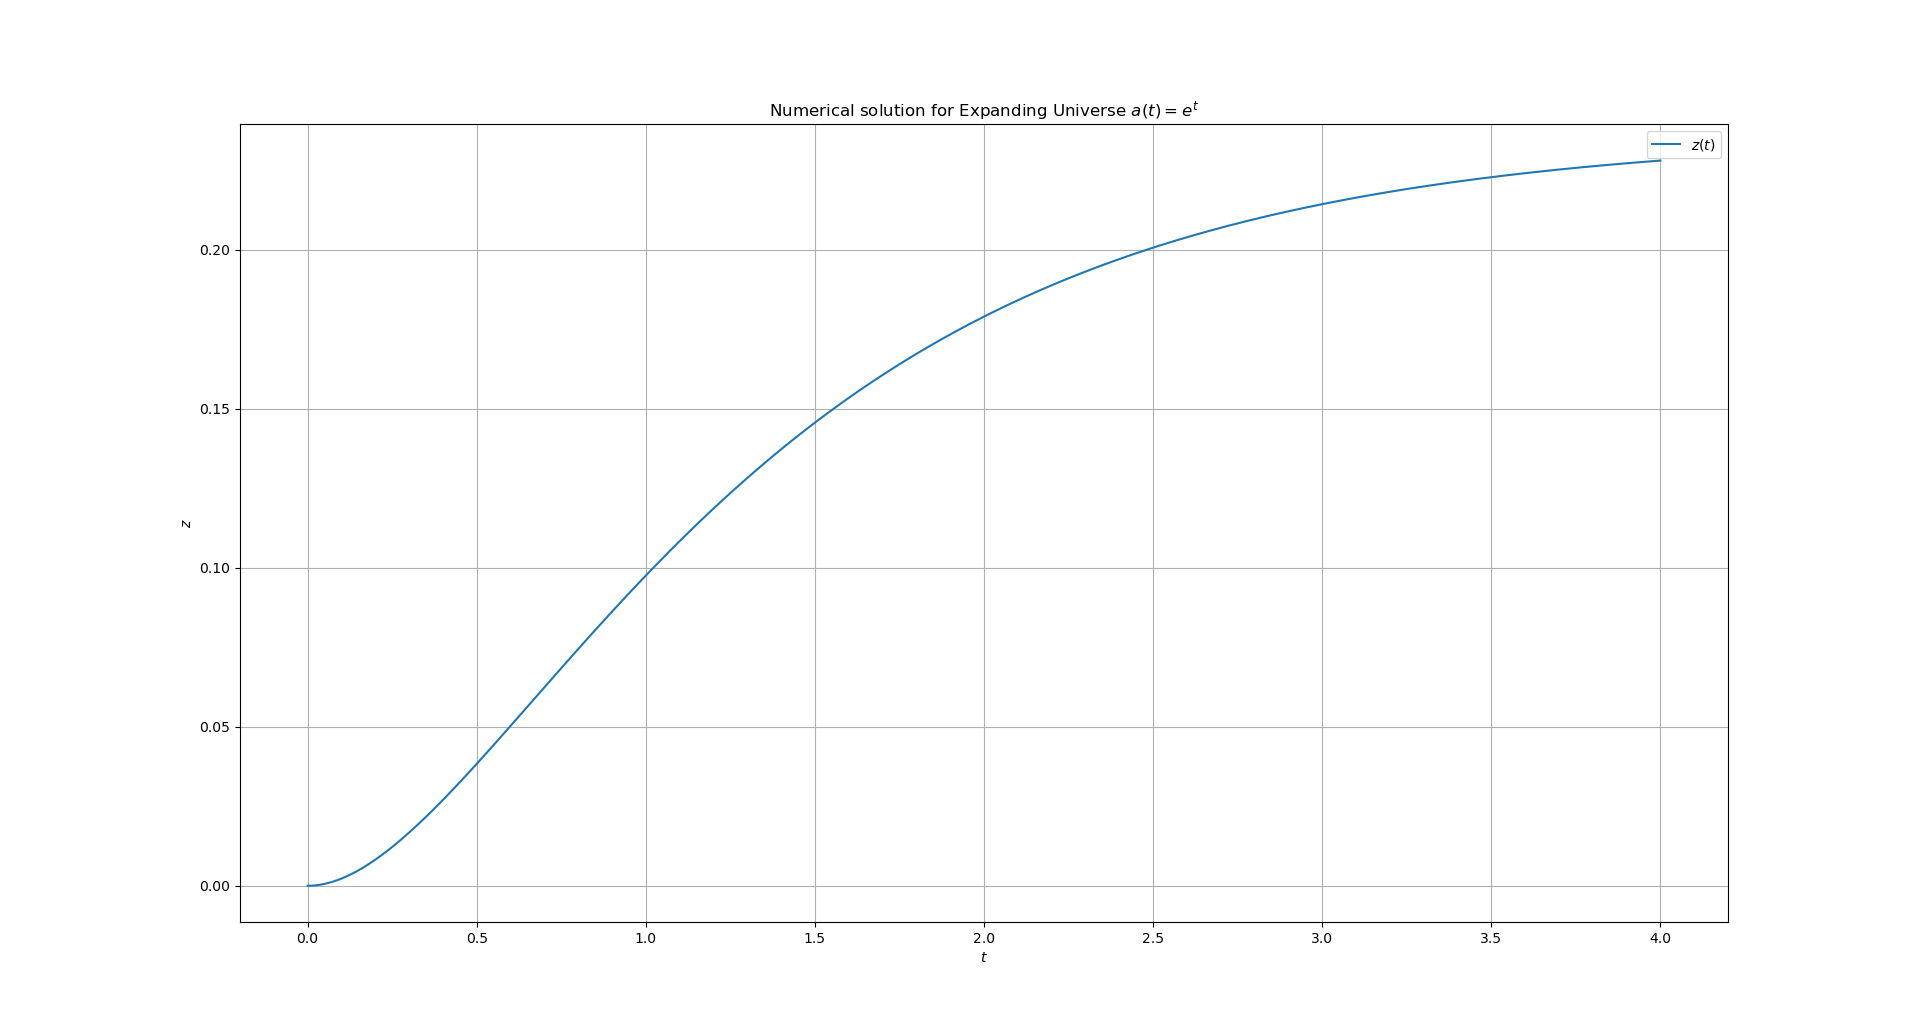
\includegraphics[scale=0.3]{./Figure_1.png}
	\centering
	\caption{Output of above program}
	\centering
\end{figure}

I also ran the program for $t\in[0,10]$; see \cref{fig:2}.
\begin{figure}[ht]
	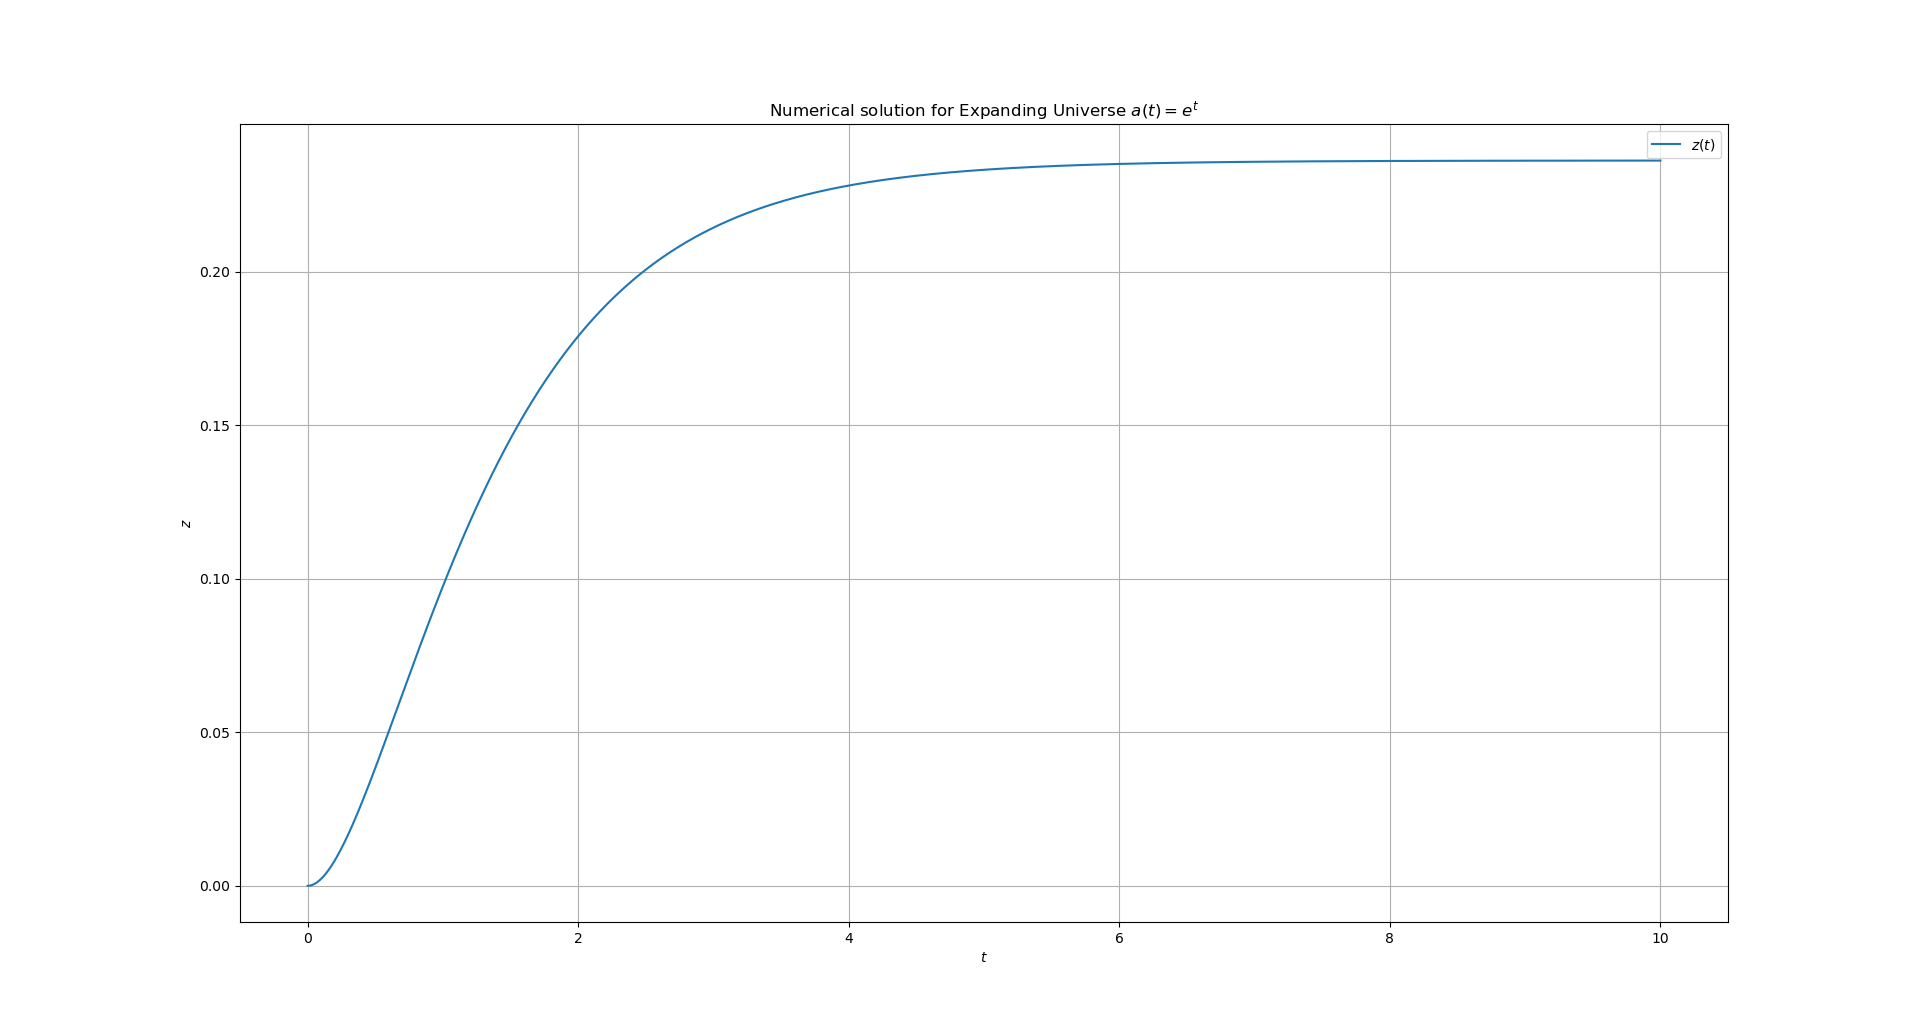
\includegraphics[scale=0.3]{./Figure_2.png}
	\centering
	\caption{Output of above program, $t$ from $0$ to $10$}\label{fig:2}
	\centering
\end{figure}

This gives a nice graph of $z(t)$. None of the behavior is too unexpected, since $e^t$ is a crazy growth rate for the universe and at $t=4$ the universe is already about $54.5$ times bigger, so we would expect that the growth should overpower the electric field in some manner. The only truly unexpected part is that the particle actually \emph{slows down} instead of just reaching zero acceleration.

Since $U^3$ looked solvable analytically, we can find the solution using sympy, which technically isn't numerics since its symbolic computation but in my opinion if a computer is doing it then its numerical.

\begin{lstlisting}[language=Python]
import sympy as sp

t = sp.Symbol('t')
E0 = 1 / 2
U3 = sp.Function('U3')
z = sp.Function('z')

eq_U3 = sp.Eq(U3(t).diff(t), E0 * sp.exp(-t) - 2 * U3(t))

eq_z = sp.Eq(z(t).diff(t), U3(t) / sp.sqrt(sp.exp(2*t) * U3(t)**2 + 1))

ivp = {
    U3(0): 0,
    z(0): 0
}

sol = sp.dsolve(
    [eq_U3, eq_z],
    [U3(t), z(t)],
    ics=ivp
)

print("U3(t):")
print(sol[0])

print("\nz(t):")
print(sol[1])
\end{lstlisting}
Output:
\begin{lstlisting}
U3(t):
Eq(U3(t), -0.5*exp(-2.0*t) + 0.5*exp(-1.0*t))

z(t):
Eq(z(t), 2.0*sqrt(0.25*(1.0*exp(1.0*t) - 1)**2*exp(-2.0*t) + 1.0) - Piecewise((-1.0*sqrt((1.0*C1 + 0.5)**2 + 1.0)/C1, Ne(C1, 0)), (-0.447213595499958, True)))
\end{lstlisting}
Writing this in LaTeX:
\[
	U^3(t)=-\frac{e^{-2t} }{2} +\frac{e^{-t} }{2} 
.\]
The $C_1$ in the expression for $z(t)$ is an artifact of the computation for $U^3$ that SymPy forgot to account for. To see this, and to see what it is equal to, we remove the IVP, let $E_0$ be an arbitrary symbol, and run it again. We get the output
\begin{lstlisting}
General U3(t):
Eq(U3(t), 1.0*C1*exp(-2.0*t) + 0.5*exp(-1.0*t))

General z(t):
Eq(z(t), C2 + Piecewise((-1.0*sqrt((1.0*C1 + 0.5*exp(1.0*t))**2*exp(-2.0*t) + 1.0)/C1, Ne(C1, 0)), (-0.447213595499958*exp(-1.0*t), True)))
also the intitial condition gives U3(0)=0: Eq(0, 1.0*C1 + 0.5)
\end{lstlisting}


We now see that $C_1=-0.5$, so $C_1\neq 0$, and thus
\[
	z(t)=2\sqrt{0.25(e^{t} -1)^2e^{-2t} +1} +\sqrt{(C1+0.5)^2+1} /C1 = 2\sqrt{\frac{e^{-2t} \left( e^t-1 \right) ^2}{4} +1} -2
.\]
Plotting this (\cref{fig:3}), we see that this is precisely the same as what was obtained earlier with numerics. So assuming I did all the algebra correctly leading up to this somehow (which I probably didn't), this is indeed an analytical answer.
\begin{figure}[ht]
	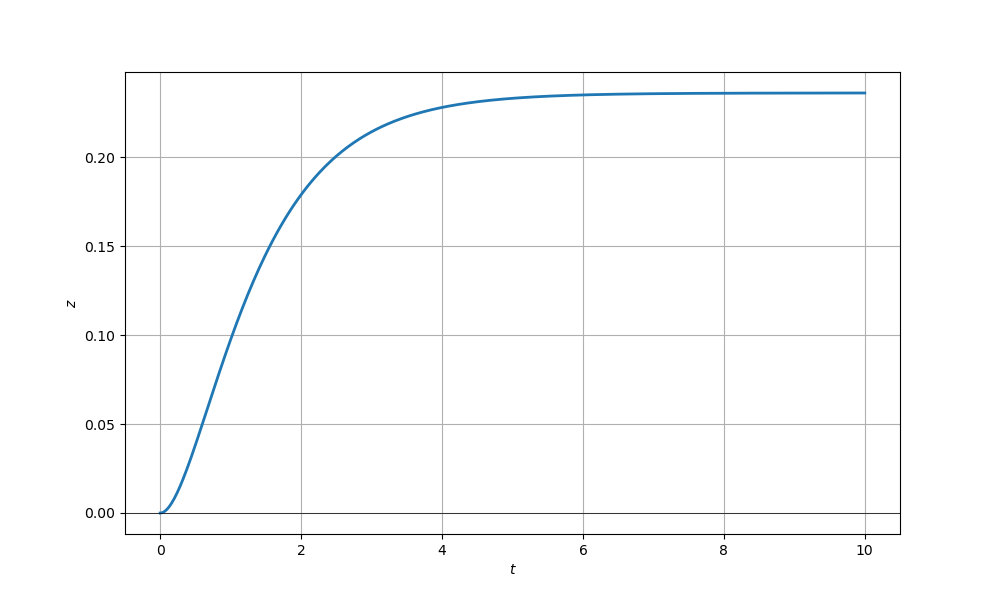
\includegraphics[scale=0.7]{./Figure_3.png}
	\centering
	\caption{Graphing the analytical solution on $t\in[0,10]$}\label{fig:3}
	\centering
\end{figure}


\section{Problem 3}
\begin{problem}
	Consider the metric
	\[
		\mathrm{d} s^2=\frac{1}{\cos ^2\rho } \left( -\mathrm{d} t^2+\mathrm{d} \rho ^2+\sin ^2\rho \mathrm{d} \theta ^2+\sin ^2\rho \sin ^2\theta \mathrm{d} \phi ^2 \right) 
	\]
	where $t$ runs from $-\infty$ to $\infty $, and $\rho ,\theta ,\phi $ are finite directions $0\leq \rho < \frac{\pi }{2} $, $0\leq \theta \leq \pi $, and $0\leq \phi <2\pi $.

	(a) Using the action principle for geodesics, find the solutions to the geodesic equation for (i) a particle with nonzero motion only in $\phi $, and (ii) a particle with nonzero motion only in $\rho $.

	(b) Now explicitly check that your solutions satisfy the geodesic equation
	\[
		\frac{\mathrm{d}^2x^\mu }{\mathrm{d}\tau ^2} +\Gamma ^\mu _{\alpha \beta } \frac{\mathrm{d}x^\alpha }{\mathrm{d}\tau } \frac{\mathrm{d}x^\beta }{\mathrm{d}\tau } =0
	.\]
\end{problem}
\noindent\textbf{Solution.} (a) The action principle for geodesics says that the Lagrangian is given by
\[
	\mathcal{L} =g_{\mu \nu } \frac{\mathrm{d}x^\mu }{\mathrm{d}\tau } \frac{\mathrm{d}x^\nu }{\mathrm{d}\tau } =g_{\mu \nu } \dot{x} ^\mu \dot{x} ^\nu ,
\]
and thus must satisfy the Euler-Lagrange equations
\[
	\frac{\mathrm{d}}{\mathrm{d}\tau } \frac{\partial \mathcal{L} }{\partial \dot{x} ^\mu } -\frac{\partial \mathcal{L} }{\partial x^\mu } =0
.\]
We see that the metric is
\[
	g_{\mu \nu } =\frac{1}{\cos ^2\rho }\operatorname{diag} (-1,1,\sin ^2\rho ,\sin ^2\rho \sin ^2\theta )
.\]
Since the metric is diagonal, off-diagonal terms vanish. We then compute the Lagrangian:
\[
	\mathcal{L} =g_{\mu \mu }\dot{x}^\mu \dot{x} ^\mu =\frac{1}{\cos ^2\rho } \left(-\frac{\mathrm{d}t}{\mathrm{d}\tau } ^2+\frac{\mathrm{d}\rho }{\mathrm{d}\tau } ^2+\sin ^2\rho \frac{\mathrm{d}\theta }{\mathrm{d}\tau } ^2+\sin ^2\rho \sin ^2\theta \frac{\mathrm{d}\phi }{\mathrm{d}\tau } ^2\right)
.\]
(i) Setting $\dot{\rho } ,\dot{\theta }=0$ gives us
\[
	\mathcal{L} =\frac{1}{\cos ^2\rho} \left( -\frac{\mathrm{d}t}{\mathrm{d}\tau } ^2+\sin ^2\rho \sin ^2\theta \frac{\mathrm{d}\phi }{\mathrm{d}\tau } ^2 \right) ,
.\]
Start with $\mu =t$. Since $\mathcal{L} $ has no $t$ dependence, $\frac{\partial \mathcal{L} }{\partial t} =0$. It follows that
\[
	\frac{\mathrm{d}}{\mathrm{d}\tau } \frac{\partial \mathcal{L} }{\partial \dot{t}} =0
.\]
Since $\mathcal{L} $ only depends on $\dot{t} ,\dot{\phi } $, we have
\[
	\frac{\partial \mathcal{L} }{\partial \dot{t} } =\frac{1}{\cos ^2\rho } \left( -2 \dot{t} \right)=-\frac{2 \dot{t} }{\cos ^2\rho } 
.\]
Since the $\tau $ derivative of this is 0, it must be constant. Since $\frac{\mathrm{d}\rho }{\mathrm{d}\tau } =0$, we have that $\rho $ is constant, meaning that $\dot{t} $ must be constant. Similarly we have
\[
	\frac{\partial \mathcal{L} }{\partial \dot{\phi } } =\frac{1}{\cos ^2\rho } \left( 2 \sin ^2\rho \sin ^2\theta \dot{\phi }  \right) 
\]
must be constant, and since $\theta ,\rho $ are constant, we have that $\dot{\phi } $ is constant. Finally, we have that since $\dot{\rho } ,\dot{\theta } =0$, $\mathcal{L} $ does not depend on these variables, so
\[
	\frac{\partial \mathcal{L} }{\partial \dot{\rho } } =\frac{\partial \mathcal{L} }{\partial \dot{\theta } } =0
.\]
It follows that
\[
	\frac{\partial \mathcal{L} }{\partial \rho } =\frac{\partial \mathcal{L} }{\partial \theta } =0
.\]
We have
\[
	\frac{\partial \mathcal{L} }{\partial \theta } =\frac{2 \sin \theta \cos \theta \sin ^2\rho }{\cos ^2\rho } \dot{\phi } ^2
.\]
For $\rho $, it's convenient to write
\[
	\mathcal{L} =\tan ^2\rho \sin ^2\theta \dot{\phi } ^2-\frac{\dot{t} ^2}{\cos ^2\rho } 
.\]
Then
\[
	\frac{\partial \mathcal{L} }{\partial \rho } =2 \tan \rho \sec ^2 \rho \sin ^2\theta \dot{\phi } ^2-\frac{2\sin \rho \dot{t} ^2}{\cos ^3\rho } =\frac{2 \sin \rho \sin ^2\theta \dot{\phi } ^2 }{\cos ^3 \rho } -\frac{2\sin \rho \dot{t} ^2}{\cos ^3\rho } =\frac{2\sin \rho }{\cos ^3\rho } \left(  \sin ^2\theta \dot{\phi } ^2-\dot{t} ^2 \right) 
.\]
Note that $\cos \rho \neq 0$ and $\dot{\phi } \neq 0$, so
\[
	\frac{\partial \mathcal{L} }{\partial \theta } =\frac{2 \sin \theta \cos \theta \sin ^2\rho }{\cos ^2\rho } \dot{\phi } ^2=0 \implies \sin \theta \cos \theta \sin ^2\rho =0
.\]
If we take $\rho =0$, then the $\dot{\phi } $ term of the Lagrangian vanishes, so the particle only has motion in time. We can thus take $\rho \neq 0$ to look for nontrivial solutions. This allows us to cancel the sin functions, giving us $\sin \theta \cos \theta =0$. This implies that $\theta $ is one of $\left\{ 0,\pi ,\pi /2 \right\} $. If $\theta $ is $0$ or $\pi $, then the $\dot{\phi } $ term in the Lagrangian once again vanishes giving us a trivial solution, so we will take $\theta =\frac{\pi }{2} $. This sets $\sin \theta =1$ and $\cos \theta =0$, and thus (recalling that $\sin \rho \neq 0$)
\[
	\frac{\partial \mathcal{L} }{\partial \rho } =\frac{2 \sin \rho }{\cos ^3\rho } \left( \dot{\phi } ^2-\dot{t} ^2 \right) =0\implies  \dot{\phi } ^2-\dot{t} ^2=0
.\]

We have that $\dot{\phi } =\pm \dot{t} $. Write $A=\dot{t} $ and $\pm A = \dot{\phi } $. Since $\dot{\phi } ,\dot{t} $ are constant,
\[
	t(\tau )=A\tau +t_0,
\]
\[
	\rho (\tau )=\rho _0,
\]
\[
	\theta (\tau )=\frac{\pi }{2} 
,\]
\[
	\phi (\tau )=\pm A\tau +\phi _0,
\]
for constants $t_0,\rho _0,\phi _0$.

(ii) Now assume that $\dot{\theta } ,\dot{\phi } $ vanish. The Lagrangian then becomes
\[
	\mathcal{L} =\frac{1}{\cos ^2\rho } \left( \dot{\rho } ^2-\dot{t} ^2 \right) 
.\]
We compute
\[
	\frac{\partial \mathcal{L} }{\partial \dot{t} } =-\frac{2 \dot{t} }{\cos ^2\rho } ,
\]
\[
	\frac{\partial \mathcal{L} }{\partial t} =0
.\]
This gives us
\[
	\frac{\mathrm{d}}{\mathrm{d}\tau } \left( -\frac{2\dot{t} }{\cos ^2\rho }  \right) =0
.\]
It follows that this is equal to some constant $A$, so we have
\[
	\dot{t} =-\frac{A \cos ^2\rho }{2} 
.\]

\[
	\frac{\partial \mathcal{L} }{\partial \dot{\rho } } =\frac{2\dot{\rho } }{\cos ^2\rho } ,
\]
\[
	\frac{\partial \mathcal{L} }{\partial \rho } =\frac{2\sin \rho }{\cos ^3\rho } \left( \dot{\rho } ^2-\dot{t} ^2 \right) 
.\]
This gives us
\[
	\frac{\mathrm{d}}{\mathrm{d}\tau } \frac{2 \dot{p} }{\cos ^2\rho } -\frac{2 \sin \rho }{\cos ^3\rho } \left( \dot{\rho } ^2-\dot{t} ^2 \right) =0
.\]
Substitute our expression for $\dot{t} $ to obtain
\[
	\frac{\mathrm{d}}{\mathrm{d}\tau } \frac{2 \dot{\rho } }{\cos ^2\rho } -\frac{2 \sin \rho }{\cos ^3\rho } \left( \dot{\rho } ^2-\frac{A^2 \cos ^4\rho }{4}  \right) =0
.\]
We have to evaluate the $\tau $-derivative.
\[
	\frac{\mathrm{d}}{\mathrm{d}\tau } \frac{2\dot{p} }{\cos ^2\rho } =\frac{2\ddot{\rho }}{\cos ^2\rho } +2\dot{\rho }\frac{\mathrm{d}}{\mathrm{d}\tau } \cos ^{-2} \rho =\frac{2\ddot{\rho }}{\cos ^2\rho } +4 \dot{\rho } \cos ^{-3} \rho \sin \rho \dot{\rho } =\frac{2\ddot{\rho }}{\cos ^2\rho } +\frac{4\dot{\rho }^2 \sin \rho }{\cos ^3\rho } 
.\]
Our equation now reads
\[
	\frac{2\ddot{\rho }}{\cos ^2\rho } +\frac{4\dot{\rho } ^2 \sin \rho }{\cos ^3\rho } -\frac{2 \sin \rho }{\cos ^3\rho } \left( \dot{\rho } ^2-\frac{A^2 \cos ^4\rho }{4}  \right) =0
.\]
Distributing and dividing out by 2 gives
\[
\frac{\ddot{\rho } }{\cos ^2\rho } +\frac{\dot{\rho } ^2 \sin \rho }{\sin \rho \cos ^3\rho } +\frac{A^2 \cos \rho }{4} =0
.\]
It will be more convenient to write
\[
	\ddot{\rho }+\dot{\rho } ^2\tan \rho +\frac{A^2}{4} \sin \rho \cos ^3\rho =0
.\]
Since the Lagrangian has no $\theta $ or $\phi $ dependence, all the relevant derivatives are zero, so we get no new information. We just define $\theta (t)=\theta _0$, $\phi (t)=\phi _0$. It now suffices to solve the differential equation for $\rho $.

The second order equation is painful to solve so we instead note that $\mathcal{L} $ has no $\tau $ dependence, so $\mathcal{L} (\tau )=C$ is some constant. Of course since $\dot{t} =-\frac{A \cos ^2\rho }{2} $, we have
\[
	\mathcal{L} =\frac{1}{\cos ^2\rho } \left( \dot{\rho } ^2-\frac{A^2 \cos ^4\rho }{2}  \right) =C
.\]
The 2 is annoying so let's define $B=A/2$. Then
\[
	\mathcal{L} =\frac{1}{\cos ^2\rho } \left( \dot{\rho } ^2-B^2 \cos ^4\rho  \right) =C
.\]
This is a first order equation, which is much easier to solve. We have
\[
	\dot{\rho } ^2=C \cos ^2\rho +B^2 \cos ^4\rho 
.\]
This is separable. We have
\[
	\frac{1}{\sqrt{C \cos ^2\rho +B^2 \cos ^4\rho } } \frac{\mathrm{d}\rho }{\mathrm{d}\tau } =1
.\]
It follows that
\[
	\int_{\rho _0}^{\rho } \frac{\mathrm{d} \rho }{\sqrt{C \cos ^2\rho +B^2 \cos ^4\rho } } =\tau 
.\]
Wolfram was able to solve the indefinite integral analytically:
\[
	\tau =\frac{\sec \rho \sqrt{\cos ^2\rho \left( C+B^2 \cos ^2 \rho  \right) } \operatorname{arctanh} \left( \frac{\sqrt{C} \sin \rho }{\sqrt{C+B^2\left( -\sin ^2\rho  \right) +B^2} }  \right) }{\sqrt{C} \sqrt{C+B^2 \cos ^2\rho } } +\text{Constant} 
.\]
I don't think it's possible to find $\rho $ as a function of $\tau $ from this, and even the series expansions are disgusting, so I will leave it at this. We have
\[
	t(\tau )=-\frac{A \cos ^2\rho }{2} ,\qquad \theta (\tau )=\theta _0,\qquad \phi (\tau )=\phi _0,\qquad \rho (\tau )=\text{numerics} 
.\]


(b) The main part of this problem is the computation of the Christoffel symbol.
\[
	\Gamma^\mu _{\alpha \beta } =\frac{1}{2} g^{\mu \sigma } \left( \frac{\partial g_{\alpha \sigma } }{\partial x^\beta } +\frac{\partial g_{\beta \sigma } }{\partial x^\alpha } -\frac{\partial g_{\alpha \beta } }{\partial x^\sigma }  \right) =\frac{1}{2} g^{\mu \mu } \left( \frac{\partial g_{\alpha \mu } }{\partial x^\beta } +\frac{\partial g_{\beta \mu } }{\partial x^\alpha } -\frac{\partial g_{\alpha \beta } }{\partial x^\mu }  \right) 
.\]
Recall $g_{\mu \nu } =\cos ^{-2} \rho \operatorname{diag} (-1,1,\sin ^2\rho ,\sin ^2\rho \sin ^2\theta )$. Then
\[
	g^{\mu \nu }=\cos ^2\rho \operatorname{diag} \left( -1,1,\frac{1}{\sin ^2\rho } ,\frac{1}{\sin ^2\rho \sin ^2\theta }  \right) 
.\]
For diagonal metrics, there is a simplification that I found \href{https://math.stackexchange.com/a/4570548}{on the internet}. We do not imply summations in the following. If $i\neq j\neq k$, then $\Gamma ^i_{jk} =0$. Otherwise,
\[
	\Gamma^i_{ii} =\frac{1}{2g_{ii} } \partial_i g_{ii} ,
\]
\[
	\Gamma^k_{ii} =-\frac{1}{2g_{kk} } \partial_kg_{ii} ,
\]
\[
	\Gamma^k_{ki} =\frac{1}{2g_{kk} } \partial _ig_{kk} 
,\]
and of course $\Gamma ^i_{jk} =\Gamma ^i_{kj} $. We start with the time component. No metric components have time dependence so $\Gamma ^0_{ii} =0$ for all $i$. We just need to compute $\Gamma ^0_{0i} $, and $g_{00} $ only has $\rho $ dependence, so we only get $\Gamma ^0_{01} $:
\[
	\Gamma ^0_{01} =-\frac{\cos ^2\rho }{2} \frac{\partial }{\partial \rho } \frac{1}{\cos ^2\rho } =\frac{\cos ^2\rho }{2} \frac{2 \sin \rho }{\cos ^3\rho } =\tan \rho 
.\]
\[
	\Gamma^0_{\alpha \beta } =\begin{pmatrix}
	0 & \tan \rho  & 0 & 0 \\
	\tan \rho  & 0 & 0 & 0 \\
	0 & 0 & 0 & 0 \\
	0 & 0 & 0 & 0
	\end{pmatrix}
.\]
$\Gamma ^1_{\alpha \beta } $ is annoying so we will do it last. Nothing else has $\phi $ dependence either so we similarly get that $\Gamma ^3_{ii} $ vanishes, so we can consider $\Gamma ^3_{3i} $. Of course $g_{33} $ only has $\rho ,\theta $ dependence so we only get contributions from $i=1,2$:
\[
	\Gamma ^3_{31} =\frac{\cos ^2\rho }{2 \sin ^2\rho \sin ^2\theta } \frac{\partial }{\partial \rho } \tan ^2\rho \sin ^2\theta =\frac{\cos ^2\rho }{2 \sin ^2\rho } 2 \tan \rho \sec ^2\rho =\frac{1}{\sin \rho \cos \rho } 
\]
\[
	\Gamma ^3_{32} =\frac{\cos ^2\rho }{2 \sin ^2\rho \sin ^2\theta } \frac{\partial }{\partial \theta } \frac{\sin ^2\rho \sin ^2\theta }{\cos ^2\rho } =\frac{1}{2 \sin ^2\theta } 2 \sin \theta \cos \theta =\frac{\cos \theta }{\sin \theta } 
.\]
\[
	\Gamma^3_{\alpha \beta } =\begin{pmatrix}
	0 & 0 & 0 & 0 \\
	0 & 0 & 0 & \frac{1}{\sin \rho \cos \rho } \\
	0 & 0 & 0 & \frac{\cos \theta }{\sin \theta }  \\
	0 & \frac{1}{\sin \rho \cos \rho }  & \frac{\cos \theta }{\sin \theta }  & 0
	\end{pmatrix}
.\]
Note that the only $g_{ii} $ with $\theta $ dependence is $i=3$, so we get
\[
	\Gamma^2_{33} =-\frac{\cos ^2\rho }{2 \sin ^2\rho } \frac{\partial }{\partial \theta } \frac{\sin ^2\rho \sin ^2\theta }{\cos ^2\rho } =-\frac{1}{2} 2 \sin \theta \cos \theta =-\sin \theta \cos \theta 
\]
Now note that $g_{22} $ only has $\rho $ dependence so
\[
	\Gamma^2_{21} =\frac{\cos ^2\rho }{2 \sin ^2\rho } \frac{\partial }{\partial \rho } \frac{\sin ^2\rho }{\cos ^2\rho } =\frac{\cos ^2\rho }{2 \sin ^2\rho } \frac{\partial }{\partial \rho } \tan ^2\rho =\frac{\cos ^2\rho }{2 \sin ^2\rho } 2 \tan \rho \sec ^2\rho =\frac{1}{\sin \rho \cos \rho } 
.\]
\[
	\Gamma^2_{\alpha \beta } =\begin{pmatrix}
	0 & 0 & 0 & 0 \\
	0 & 0 & \frac{1}{\sin \rho \cos \rho }  & 0 \\
	0 & \frac{1}{\sin \rho \cos \rho }  & 0 & 0 \\
	0 & 0 & 0 & -\sin \theta \cos \theta 
	\end{pmatrix}
.\]
Finally, every term has $\rho $ dependence so we must compute all of the form $\Gamma ^1_{ii} $. However, $g_{11} $ only has $\rho $ dependence, so the $\Gamma ^1_{1i} $ term is accounted for by $\Gamma ^1_{11} $.
\[
	\Gamma^1_{00} =-\frac{\cos ^2\rho }{2} \frac{\partial }{\partial \rho } \left( -\sec ^2\rho  \right) =\frac{\cos ^2\rho }{2} 2 \sec ^2\rho \tan \rho =\tan \rho 
.\]
\[
	\Gamma^1_{11} =-\frac{\cos ^2\rho }{2} \frac{\partial }{\partial \rho } \sec ^2\rho =-\tan \rho 
.\]
\[
	\Gamma^1_{22} =-\frac{\cos ^2\rho }{2} \frac{\partial }{\partial \rho } \tan ^2\rho =-\frac{\cos ^2\rho }{2} 2 \tan \rho \sec ^2\rho =-\tan \rho 
.\]
\[
	\Gamma^1_{33} =-\frac{\cos ^2\rho }{2} \frac{\partial }{\partial \rho } \frac{\sin ^2\rho \sin ^2\theta }{\cos ^2\rho } =-\sin ^2\theta \tan \rho 
.\]
We get
\[
	\Gamma^1_{\alpha \beta } =\begin{pmatrix}
	\tan \rho   & 0 & 0 & 0 \\
	0 & - \tan \rho  & 0 & 0 \\
	0 & 0 & -\tan \rho  & 0 \\
	0 & 0 & 0 & -\sin ^2\theta \tan \rho 
	\end{pmatrix}
.\]

(i) Recall our system
\[
	t(\tau )=A\tau +t_0,\qquad \rho (\tau )=\rho _0,\qquad \theta (\tau )=\frac{\pi }{2} ,\qquad \phi (\tau )=\pm A\tau +\phi _0
.\]
All of the second derivatives with respect to $\tau $ vanish, so the geodesic equation reads
\[
	\Gamma_{\alpha \beta } ^\mu \frac{\mathrm{d}x^\alpha }{\mathrm{d}\tau } \frac{\mathrm{d}x^\beta }{\mathrm{d}\tau } =0
.\]
For $\mu =0$, we only consider the derivatives of $t$ and $\rho $ because $\Gamma^0_{10} =\tan \rho $ and 0 elsewhere. We have
\[
	\frac{\mathrm{d}t}{\mathrm{d}\tau } =A,\qquad \frac{\mathrm{d}\rho }{\mathrm{d}\tau } =0
.\]
Since the derivative of $\rho $ vanishes, both terms vanish. Now take $\mu =1$. The matrix is diagonal, and the derivatives of $\rho ,\theta $ vanish, so we consider only $t$ and $\phi $ derivatives, which are $A$ and $\pm A$, respectively. We have
\[
	\Gamma^1_{\alpha \beta } \frac{\mathrm{d}x^\alpha }{\mathrm{d}\tau } \frac{\mathrm{d}x^\beta }{\mathrm{d}\tau } =\pm A^2 \tan \rho -(\pm A^2) \sin ^2 \tan \rho 
.\]
Since $\theta =\pi /2$, $\sin \theta =1$, so the two terms cancel. Now take $\mu =2$. Two of the nonvanishing terms in $\Gamma^2_{\alpha \beta } $ have derivatives of $\rho $ and $\theta $ in the geodesic equation, both of which vanish, and $\cos \theta =0$ so $\Gamma^2_{33} =0$. Therefore, that term vanishes. Finally, $\Gamma^0_{\alpha \beta } $ once again only has nonzero terms at entries corresponding to derivatives of $\rho $, so those vanish. Therefore, the geodesic equation is satisfied.


(ii) Recall our system
\[
	t(\tau )=-\frac{A \cos ^2\rho }{2},\qquad \theta (\tau )=\theta _0,\qquad \phi (\tau )=\phi _0,
\]
and we will reference results about $\rho $ when needed. For example,
\[
	\frac{\mathrm{d}^2\rho }{\mathrm{d}\tau ^2} =-\frac{\mathrm{d}\rho }{\mathrm{d}\tau } ^2 \tan \rho -\frac{A^4}{4} \sin \rho \cos ^3 \rho 
.\]
We will need this when taking $\mu =1$. Note that the second derivatives vanishes for $\mu =2,3$ so
\[
	\Gamma ^\mu_{\alpha \beta } \frac{\mathrm{d}x^\alpha }{\mathrm{d}\tau } \frac{\mathrm{d}x^\beta }{\mathrm{d}\tau } =0,\qquad \mu \neq 0,1
.\]
Start with $\mu =0$. We get
\[
	\ddot{t} +2 \tan \rho \dot{t} \dot{\rho } =\ddot{t} -A \cos ^2\rho \tan \rho \dot{\rho } =0
.\]
We have
\[
	\frac{\mathrm{d}\dot{t} }{\mathrm{d}\tau } =\frac{\mathrm{d}}{\mathrm{d}\tau } -\frac{A \cos ^2\rho }{2} =2\frac{A \cos \rho }{2} \sin \rho \dot{\rho } =A \cos ^2\rho \tan \rho \dot{\rho } 
.\]
Therefore, the geodesic equation is satisfied for this case. For $\mu =1$, we only have contributions from the first two terms giving
\[
	\ddot{\rho } + \dot{t}^2 \tan \rho +\dot{\rho } ^2 \tan \rho =0 
.\]
Indeed, recall that
\[
	\ddot{\rho } +\dot{\rho } ^2 \tan \rho +\frac{A^2}{4} \sin \rho \cos ^3\rho =0
.\]
Substituting in $\dot{t} =-\frac{1}{2} A \cos ^2\rho $ and doing some algebra gives
\[
	\ddot{\rho } +\dot{\rho } ^2 \tan \rho +\frac{A^2}{4} \sin \rho \cos ^3\rho =0
.\]
We have already seent hat this equation is satisfied. Therefore, $\mu =1$ satisfies the geodesic equation.


Derivatives of $\theta $ and $\phi $ vanish, and every term of $\Gamma^2_{\alpha \beta } $ contains a derivative of one of them. Therefore, the $\mu =2$ term vanishes. Similarly, every term in the $\mu =3$ part of the Christoffel corresponds to a derivative of $\phi $ so that vanishes. Therefore the geodesic equation is satisfied.








\newpage
\section{AI response for problem 2}

For numerically solving systems of differential equations, **Python** is the standard and most effective choice due to its extensive scientific computing ecosystem.

The primary packages you will need are:
* **NumPy**: For efficient handling of arrays and basic numerical operations.
* **SciPy**: For the core integration routines. Specifically, the `scipy.integrate.solve\_ivp` function is the modern, recommended tool for solving initial value problems for systems of ODEs.
* **Matplotlib**: For plotting and visualizing the results.

---

\#\# Workflow and Example

The general process involves defining your system of differential equations as a Python function, setting initial conditions, and then passing these to the solver.

Let's solve the following system for a simple harmonic oscillator:
$$
\begin{cases}
\frac{dx}{dt} = v \\
\frac{dv}{dt} = -x
\end{cases}
$$
Here, the state of the system is represented by the vector $y = [x, v]$. The derivative of the state vector is $\frac{dy}{dt} = \left[ \frac{dx}{dt}, \frac{dv}{dt} \right] = [v, -x]$.

\#\#\# Python Implementation

Here is a complete example of how to implement and solve this system:
\begin{lstlisting}[language=Python]
import numpy as np
from scipy.integrate import solve_ivp
import matplotlib.pyplot as plt

# 1. Define the system of differential equations
# The function must take t (time) and y (the state vector [x, v]) as arguments.
def harmonic_oscillator(t, y):
    """
    Defines the derivatives for a simple harmonic oscillator.
    y[0] = x (position)
    y[1] = v (velocity)
    Returns [dx/dt, dv/dt]
    """
    dydt = [y[1], -y[0]]
    return dydt

# 2. Set initial conditions and time span
# Initial state: x(0) = 1, v(0) = 0
y0 = [1.0, 0.0]

# Time span: solve from t=0 to t=10
t_span = [0, 10]
# Specify times at which to store the solution
t_eval = np.linspace(t_span[0], t_span[1], 101)

# 3. Solve the ODE system
# solve_ivp returns a solution object
sol = solve_ivp(
    fun=harmonic_oscillator, 
    t_span=t_span, 
    y0=y0, 
    t_eval=t_eval
)

# 4. Extract and plot the results
t = sol.t
x = sol.y[0] # Position is the first component of the solution vector
v = sol.y[1] # Velocity is the second component

plt.figure(figsize=(10, 6))
plt.plot(t, x, label='Position (x)')
plt.plot(t, v, label='Velocity (v)')
plt.title('Simple Harmonic Oscillator')
plt.xlabel('Time (t)')
plt.ylabel('Value')
plt.grid(True)
plt.legend()
plt.show()
\end{lstlisting}

\#\#\# Explanation of `solve\_ivp` Arguments

* `fun`: The function defining the system of ODEs.
* `t\_span`: A 2-element sequence `(t\_start, t\_end)` specifying the interval of integration.
* `y0`: The initial state vector at `t\_start`.
* `t\_eval`: An array of time points where you want the solution to be stored. If not provided, the solver chooses its own steps. It's good practice to provide this for clean plotting.

This setup can be easily extended to more complex, higher-dimensional systems by increasing the size of the state vector `y` and defining the corresponding derivatives in your function.
\end{document}
